\documentclass{article}

\usepackage{amsmath,amssymb}
\usepackage[superscript]{cite}
\usepackage{cleveref}
\usepackage{tikz}
\usetikzlibrary{arrows.meta}

\newcommand{\bra}[1]{\ensuremath{\left\langle#1\right|}}
\newcommand{\ket}[1]{\ensuremath{\left|#1\right\rangle}}
\newcommand{\ensb}[1]{\left\langle#1\right\rangle}
\newcommand{\comm}[2]{\left[#1,#2\right]}
\newcommand{\vect}[1]{\ensuremath{\boldsymbol{\mathbf{#1}}}}
\newcommand{\tr}[1]{\ensuremath{\mathrm{~Tr}\left[#1\right]}}
\newcommand{\trb}[1]{\ensuremath{\mathrm{~Tr_{b}}\left[#1\right]}}
\newcommand{\ensbb}[1]{\left\langle#1\right\rangle_{b}}
\newcommand{\arw}{-{Latex[length=2mm]}}

\begin{document}

\title{Third-Order Response Functions in the Semiclassical Approximation}
\author{Nicholas Hestand}
\date{\today}
\maketitle

These notes contain the derivation of the first and third order response functions for coupled chromophores in a semiclassical approximation.
The derivation follows closely that given by Mukamel for a two-level system,\cite{Mukamel1995} but extended to account for multiple chromphores as in reference \citenum{Auer2007} for the linear response function.
We consider $N$ three-level chromophores that are coupled to bath degrees of freedom \vect{q}.
At a given time, any number of these chromophores can be in either their ground state, first excited state, or second excited state.
We define the global ground state as $$\ket{G}=\ket{1_{g},2_{g},...,N-1_{g},N_{g}},$$ a one-exciton state as $$\ket{n_{1}}=\ket{1_{g},2_{g},...,n_{1},...,N-1_{g},N_{g}},$$ and a two-exciton state as either $$\ket{n_{2}}=\ket{1_{g},2_{g},...,n_{2},...,(N-1)_{g},N_{g}}$$ or $$\ket{n_{1},m_{1}}=\ket{1_{g},2_{g},...,n_{1},...,m_{1}...,(N-1)_{g},N_{g}}.$$
Here the notation $n_{m}$ denotes that chromophore $n$ is in state $m=\{g,1,2\}$.
Note that there are two types of two-exciton states, one where two different chromophores are excited and one where a single chromophore is doubly excited.
Higher exciton states (i.e. three-exciton, four-exciton, etc.) also exist, but they will not be important for the first- or third-order response functions so we will ignore them here.

The adiabatic Hamiltonian for the system is given by
\begin{equation}
\begin{split}
 H&=\ket{G}H_{G}^{0}(\vect{q})\bra{G}+\sum_{i,j=1}^{N}\ket{i_{1}}H^{1}_{ij}(\vect{q})\bra{j_{1}}\\
 &+\sum_{i,j=1}^{N}\ket{i_{2}}H_{ij}^{2}(\vect{q})\bra{j_{2}}+\sum_{i>j,k>l=1}^{N}\ket{i_{1},j_{1}}H_{ijkl}^{2}(\vect{q})\bra{k_{1},l_{1}}\\
 &+\sum_{i=1,j>k=1}^{N}\ket{i_{2}}H_{ijk}^{2}(\vect{q})\bra{j_{1},k_{1}}+\ket{j_{1},k_{1}}H_{ijk}^{2}(\vect{q})\bra{i_{2}}.
\end{split}
\end{equation}
In the exciton space, the first term acts on the global ground state, the second on the one-exciton states and the remaining three on the two-exciton states.
The limits on the summations ensure that there is no double counting in the two-exciton subspace.
Note that the Hamiltonians $H_{G}^{0}(\vect q)$, $H_{ij}^{1}(\vect q)$, ..., are matrix elements in the exciton basis, but operators on the bath degrees of freedom, \vect{q}.
This is important!
Finally, note that the ground, one-exciton, and two-exciton subspaces are uncoupled.
Given this Hamiltonian, we can derive the response functions of interest.

\section{First-Order Response Function}
The first-order (linear) response function for a system at time $\tau_{1}$ interacting with a laser pulse at time $\tau_{0}$ is given by\cite{Mukamel1995,Hamm2011}
\begin{equation}
\begin{split}
S^{(1)}(\tau_{1})&=\frac{i}{\hbar}\theta(\tau_{0})\ensb{\vect\epsilon(\tau_{1})\cdot\vect\mu(\tau_{1})\comm{\vect\epsilon(\tau_{0})\cdot\vect\mu(\tau_{0})}{\rho(-\infty)}}\\
&=\frac{i}{\hbar}\theta(\tau_{0})\left(R^{(1)}(t_{1})-R^{(1)*}(t_{1})\right)
\end{split}
\end{equation}
with
\begin{equation}
\label{eq:R1}
R^{(1)}(t_{1})=\ensb{\vect\epsilon(t_{1})\cdot\vect\mu(t_{1})\vect\epsilon(0)\cdot\vect\mu(0)\rho(-\infty)}.
\end{equation}
Here, $\vect\epsilon(t_{1})$ is the unit vector pointing along the direction of the light polarization vector at time $t_{1}$, $\theta(\tau)$ is the Heavyside step function, $\rho(-\infty)=\exp[-\beta H]/\ensb{\exp[-\beta H]}$ ($\beta=1/kT$) and $R^{(1)*}(t_{1})$ is the complex conjugate of $R^{(1)}(t_{1})$.
The variable $t_{1}=\tau_{1}-\tau_{0}$ is the relative time after the system interacts with the light pulse.
The Heavyside function, defined by $\theta(\tau)= 0$ if $\tau <0$ and 1 if $\tau>=0$, enforces causality since the system cannot respond to the light pulse before first interacting with it at $\tau_{0}$.
The transition dipole moment at time $t_{1}$ is given in the Heisenberg representation by
\begin{equation}
\vect\mu(t_{1})=e^{iHt_{1}/\hbar}\vect\mu e^{-iHt_{1}/\hbar}.
\end{equation}
$\vect{\mu}$ is expanded in the exciton basis as
\begin{equation}
\begin{split}
\hat{\vect{\mu}}&=\sum_{n}\vect\mu_{n_{g1}}(\vect q)\left(\ket{n_{g}}\bra{n_{1}}+\ket{n_{1}}\bra{n_{g}}\right)\\
		&+\sum_{n}\vect\mu_{n_{12}}(\vect q)\left(\ket{n_{1}}\bra{n_{2}}+\ket{n_{2}}\bra{n_{1}}\right)\\
		&+\sum_{n,m}\vect\mu_{m_{g1}}(\vect q)\left(\ket{n_{1},m_{1}}\bra{n_{1}}+\ket{n_{1}}\bra{n_{1},m_{1}}\right),
\end{split}
\end{equation}
where $\vect\mu_{n_{g1}}(\vect q)$ and $\vect\mu_{n_{12}} (\vect q)$ are the ground-to-one and one-to-two exciton transition dipole moments for chromophore $n$.
Note that these are matrix elements in the exciton subspace but operators on the bath degrees of freedom, \vect{q}.
Finally, in \Cref{eq:R1} $\left\langle \ldots \right\rangle$ denote a trace over all system and bath degrees of freedom.

If we assume that the one-exciton energy is much greater than $kT$ and expand $\rho(-\infty)$ in the exciton basis, we have
\begin{equation}
\rho(-\infty)\sim \ket{G}e^{-\beta H_{G}^{0}(\vect{q})}\bra{G}/\ensb{e^{-\beta H_{G}^{0}(\vect{q})}}.
\end{equation}
Inserting this expression into \Cref{eq:R1} and expanding in the exciton basis, we have
\begin{equation}
\begin{split}
R^{(1)}(t_{1})&\sim
\left\langle e^{iH_{G}^{0}(\vect q)t_{1}/\hbar}\times\right. \\
&\sum_{m}\vect\epsilon(t_{1})\cdot\vect\mu_{m_{g1}}(\vect q)\bra{m_{1}}
e^{-i\sum_{a,b}\ket{a_{1}}H_{ab}^{1}(\vect q)\bra{b_{1}} t_{1}/\hbar}
\sum_{n}\vect\epsilon(0)\cdot\vect\mu_{n_{g1}}(\vect q)\ket{n_{1}}\times\\
&\left. e^{-\beta H_{G}^{0}(\vect{q})}\right\rangle/\ensb{e^{-\beta H_{G}^{0}(\vect{q})}}.
\end{split}
\end{equation}
We now introduce the collective bath coordinate $U_{ij}^{1}(\vect q)=H_{ij}^{1}(\vect q)-H_{G}^{0}(\vect q)\delta_{ij}$, which is in the Heisenberg representation
\begin{equation}
U_{ij}^{1}(\vect q, t)=e^{itH(\vect q)/\hbar}U_{ij}^{1}(\vect q)e^{-itH(\vect q)/\hbar}.
\end{equation}
Now, following reference \citenum{Mukamel1995} and taking $H_{G}^{0}(\vect q)$ as our reference Hamiltonian, we can write
%see p 204
\begin{equation}
e^{-i\sum_{a,b}\ket{a_{1}}H_{ab}^{1}(\vect q)\bra{b_{1}} t_{1}/\hbar}=e^{-iH_{G}^0(\vect q)t_{1}/\hbar}\exp_{+}\left[-i/\hbar\int_0^{t_1}d\tau\sum_{ab}\ket{a_{1}}\bar U_{ab}(\tau,\vect q) \bra{b_{1}}\right]
\end{equation}
where 
\begin{equation}
\bar{U}_{ij}^{1}(\vect q, t)=e^{itH_{G}^{0}(\vect q)/\hbar}U_{ij}^{1}(\vect q)e^{-itH_{G}^{0}(\vect q)/\hbar}
\end{equation}
is the $U_{ij}$ operator in the interaction picture with respect to the ground state Hamiltonian.
Furthermore $\exp_{+}{\left[\int_{0}^{t}\ldots \right]}$ is the time-ordered exponential.\cite{Mukamel1995}
Subbing this into our expression for $R^{(1)}$ we have
\begin{equation}
\begin{split}
R^{(1)}(t_{1})&\sim
\left\langle e^{iH_{G}^{0}(\vect q)t_{1}/\hbar}\times\right. \\
&\sum_{m}\vect\epsilon(t_{1})\cdot\vect\mu_{m_{g1}}(\vect q)e^{-iH_{G}^0(\vect q)t_{1}/\hbar}\bra{m_{1}}
\exp_{+}\left[-i/\hbar\int_0^{t_1}d\tau\sum_{ab}\ket{a_{1}}\bar U_{ab}(\tau,\vect q) \bra{b_{1}}\right]\times\\
&\sum_{n}\vect\epsilon(0)\cdot\vect\mu_{n_{g1}}(\vect q)\ket{n_{1}}\times
\left. e^{-\beta H_{G}^{0}(\vect{q})}\right\rangle/\ensb{e^{-\beta H_{G}^{0}(\vect{q})}}.
\end{split}
\end{equation}
Defining the time evolution of the dipole operators with respect to the ground state Hamiltonian as
\begin{equation}
\vect \mu_{m_{g,1}}(t,\vect q)=
e^{iH_{G}^{0}(\vect q)t/\hbar}\vect\mu_{m_{g1}}(\vect q)e^{-iH_{G}^0(\vect q)t/\hbar},
\end{equation}
the response function becomes
\begin{equation}
\begin{split}
R^{(1)}(t_{1})&\sim
\left\langle\sum_{m}\vect\epsilon(t_{1})\cdot \vect \mu_{m_{g,1}}(t_{1},\vect q) \bra{m_{1}}
\exp_{+}\left[-i/\hbar\int_0^{t_1}d\tau\sum_{ab}\ket{a_{1}}\bar U_{ab}(\tau,\vect q) \bra{b_{1}}\right]\times\right.\\
&\sum_{n}\vect\epsilon(0)\cdot\vect \mu_{n_{g,1}}(0,\vect q)\ket{n_{1}}\times
\left. e^{-\beta H_{G}^{0}(\vect{q})}\right\rangle/\ensb{e^{-\beta H_{G}^{0}(\vect{q})}}.
\end{split}
\end{equation}
Finally, we make the semiclassical approximation. 
First, the dynamics of the bath operators $\bar U_{ab}(\tau,\vect q)$ and $\vect \mu(t,\vect q)$ are replaced by classical dynamical trajectories on the ground state potential.
The matrix elements in the exciton space then become functions of the classical bath coordinates, 
\begin{equation}
\begin{split}
\bar U_{ab}(t,\vect q)&\rightarrow \bar U_{ab}[\vect q(t)]=\hbar\omega_{a}[\vect q(t)]\delta_{ab} + \hbar\omega_{ab}[\vect q(t)](1-\delta_{ab})\\
\vect\mu_{m_{g,1}}(t,\vect q)&\rightarrow \vect\mu_{m_{g,1}}[\vect q(t)]
\end{split}
\end{equation}
where $\hbar \omega_{a}[\vect q(t)]$ is the fluctuating transition energy from the ground to first excited state of chromophore $a$, and $\hbar\omega_{ab}[\vect q(t)]$ is the fluctuating coupling between chromophores $a$ and $b$. 
Since $\bar U_{ab}$ is now treated as a classical variable rather than an operator, we can write the time ordered exponential as a regular integral.
Finally, the trace $\ensb{\ldots e^{-\beta H_{G}^{0}(\vect q)}}/\ensb{e^{-\beta H_{G}^{0}(\vect q)}}$ is replaced by a classical Boltzmann bath average over initial conditions.
We then have
\begin{equation}
\begin{split}
R^{(1)}(t_{1})\sim
&\left\langle\sum_{m}\vect\epsilon(t_{1})\cdot \vect\mu_{m_{g,1}}[\vect q(t_{1})] \bra{m_{1}}
\exp\left[-i/\hbar\int_0^{t_1}d\tau\sum_{ab}\ket{a_{1}}\bar U_{ab}[\vect q(\tau)] \bra{b_{1}}\right]\times\right.\\
&\left. \sum_{n}\ket{n_{1}}\vect\epsilon(0)\cdot\vect\mu_{n_{g,1}}[\vect q(0)] \right\rangle_{b}.
\end{split}
\end{equation}
If we let \underline{$\vect M$}$[\vect q(t)]=\sum_{m}\vect\epsilon(t)\cdot \vect\mu_{m_{g,1}}[\vect q(t)] \bra{m_{1}}$ be a $1\times N$ vector and if we let \underline{$\vect H$}$^{1}[\vect q(t)]=\sum_{ab}\ket{a_{1}}\bar U_{ab}[\vect q(t)]\bra{b_{1}}$ be a $N\times N$ matrix, we can write the response function in a more compact notation as
\begin{equation}
R^{(1)}(t_{1})\sim\left\langle \underbar{\vect{M}}^{T}[\vect q(t_{1})]\exp\left[i/\hbar\int_{0}^{t_{1}}\underbar{\vect{H}}^{1}[\vect q(\tau)]d\tau\right] \underbar{\vect{M}} [\vect q(0)] \right\rangle_{b}.
\end{equation}
This equation can be evaluated numerically in a straightforward manner.
\Cref{fig:fd1} shows the two-sided Feynman diagram corresponding to $R^{(1)}$.

\begin{figure}
\centering
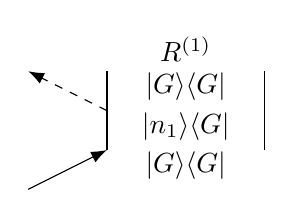
\begin{tikzpicture}[x=.5cm,y=.5cm]
\node[above] at (2, 2) {$R^{(1)}$};
%stimulated emission
\draw (0,0) -- (0,2);
\draw (4,0) -- (4,2);
\draw[\arw] (-2,-1) -- (0 ,0);
\draw[dashed,\arw] (0 , 1) -- (-2, 2);
\node[above] at (2,-1) {\ket{G}\bra{G}};
\node[above] at (2, 0) {\ket{n_{1}}\bra{G}};
\node[above] at (2, 1) {\ket{G}\bra{G}};
\end{tikzpicture}
\caption{Double sided Feynman diagram for $R^{(1)}$.}\label{fig:fd1}
\end{figure}


\section{Third-Order Response Function}
We can use the same general technique to derive the third-order response functions in a semiclassical approximation.
The third-order response function for a system interacting with laser pulses at time $\tau_{0}$, $\tau_{1}$ and $\tau_{2}$ is given by\cite{Mukamel1995,Hamm2011}
\begin{equation}
\begin{split}
S^{(3)}(\tau_{1},\tau_{2},\tau_{3})&\\
 =\left(\frac{i}{\hbar}\right)^{3}&\theta(\tau_{0})\theta(\tau_{1})\theta(\tau_{2})
 \ensb{\vect\epsilon\cdot\vect\mu(t_{3})
 \comm{\vect\epsilon\cdot\vect\mu(t_{2})}{
 \comm{\vect\epsilon\cdot\vect\mu(t_{1})}{
 \comm{\vect\epsilon\cdot\vect\mu(t_{0})}{
 \rho(-\infty)}}}}\\
 =\left(\frac{i}{\hbar}\right)^{3}&\theta(\tau_{0})\theta(\tau_{1})\theta(\tau_{2})\times\\
            &\left\langle R^{(3)}_{1}(t_{1},t_{2},t_{3})-R^{(3)*}_{1}(t_{1},t_{2},t_{3})\right.\\
            &+R^{(3)}_{2}(t_{1},t_{2},t_{3})-R^{(3)*}_{2}(t_{1},t_{2},t_{3})\\ 
            &+R^{(3)}_{3}(t_{1},t_{2},t_{3})-R^{(3)*}_{3}(t_{1},t_{2},t_{3})\\
            &\left.+R^{(3)}_{4}(t_{1},t_{2},t_{3})-R^{(3)*}_{4}(t_{1},t_{2},t_{3})\right\rangle
\end{split}
\end{equation}
Here $R_{n}^{(3)*}$ is just the complex conjugate of $R_{n}^{(3)}$ and $t_{n}=\tau_{n}-\tau_{n-1}$ is the relative times between successive light pulses.
The four $R^{(3)}$ functions are given by
\begin{equation}
\begin{split}
R_{1}^{(3)}(t_{1},t_{2},t_{3})=&\left\langle\vect{\epsilon}(t_{1})\cdot\vect{\mu}(t_{1})
				     \vect{\epsilon}(t_{1}+t_{2})\cdot\vect{\mu}(t_{1}+t_{2})\times\right.\\
				     &\left.\vect{\epsilon}(t_{1}+t_{2}+t_{3})\cdot\vect{\mu}(t_{1}+t_{2}+t_{3})
				     \vect{\epsilon}(0)\cdot\vect{\mu}(0)
				     \rho(-\infty)\right\rangle\\
R_{2}^{(3)}(t_{1},t_{2},t_{3})=&\left\langle\vect{\epsilon}(t_{0})\cdot\vect{\mu}(t_{0})
				     \vect{\epsilon}(t_{1}+t_{2})\cdot\vect{\mu}(t_{1}+t_{2})\times\right.\\
				     &\left.\vect{\epsilon}(t_{1}+t_{2}+t_{3})\cdot\vect{\mu}(t_{1}+t_{2}+t_{3})
				     \vect{\epsilon}(t_{1})\cdot\vect{\mu}(t_{1})
				     \rho(-\infty)\right\rangle\\
R_{3}^{(3)}(t_{1},t_{2},t_{3})=&\left\langle\vect{\epsilon}(t_{0})\cdot\vect{\mu}(t_{0})
				     \vect{\epsilon}(t_{1})\cdot\vect{\mu}(t_{1})\times\right.\\
				     &\left.\vect{\epsilon}(t_{1}+t_{2}+t_{3})\cdot\vect{\mu}(t_{1}+t_{2}+t_{3})
				     \vect{\epsilon}(t_{1}+t_{2})\cdot\vect{\mu}(t_{1}+t_{2})
				     \rho(-\infty)\right\rangle\\
R_{4}^{(3)}(t_{1},t_{2},t_{3})=&\left\langle\vect{\epsilon}(t_{1}+t_{2}+t_{3})\cdot\vect{\mu}(t_{1}+t_{2}+t_{3})
				     \vect{\epsilon}(t_{1}+t_{2})\cdot\vect{\mu}(t_{1}+t_{2})\times\right.\\
				     &\left.\vect{\epsilon}(t_{1})\cdot\vect{\mu}(t_{1})
				     \vect{\epsilon}(0)\cdot\vect{\mu}(0)
				     \rho(-\infty)\right\rangle\\
\end{split}
\end{equation}

We now expand these, one by one, in the exciton basis assuming that the one-exciton energy is much greater than $kT$.
For $R_{1}^{(3)}$ we have
\begin{equation}
\begin{split}
R_{1}^{(3)}(t_{1},t_{2},t_{3})=
%t1
&\left \langle e^{iH_{G}^{0}(\vect q)t_{1}}\sum_{k}\vect{\epsilon}(t_{1})\cdot\vect\mu_{k_{g1}}(\vect q)\bra{k_{1}}\right.\\
%t1+t2
&\times e^{i\sum_{a,b}\ket{a_{1}}H_{ab}^{1}(\vect q)\bra{b_{1}}t_{2}/\hbar}\sum_{l}\vect\epsilon(t_{1}+t_{2})\cdot\vect\mu_{l_{g1}}(\vect q)\ket{l_{1}}\\
%t1+t2+t3
&\times e^{iH_{G}^{0}(\vect q)t_{3}/\hbar}\sum_{m}\vect\epsilon(t_{1}+t_{2}+t_{3})\cdot\vect\mu_{m_{g1}}(\vect q)\bra{m_{1}}\\
&\times e^{-i\sum_{a,b}\ket{a_{1}}H_{ab}^{1}(\vect q)\bra{b_{1}}(t_{3}+t_{2}+t_{1})/\hbar}\\
&\left. \times \sum_{n}\vect\epsilon(0)\cdot\vect\mu_{n_{g1}}(\vect q)\ket{n_{1}}
\times e^{-\beta H_{G}^{0}(\vect{q})}\right\rangle/\ensb{e^{-\beta H_{G}^{0}(\vect{q})}}\\
% to excited state
+&\left \langle e^{iH_{G}^{0}(\vect q)t_{1}}\sum_{k}\vect{\epsilon}(t_{1})\cdot\vect\mu_{k_{g1}}(\vect q)\bra{k_{1}}\right.\\
%t1+t2
&\times e^{i\sum_{a,b}\ket{a_{1}}H_{ab}^{1}(\vect q)\bra{b_{1}}t_{2}/\hbar}\vect\epsilon(t_{1}+t_{2})\cdot\\
&\sum_{l}\ket{l_{1}}\left(\sum_{x\ne l}\vect\mu_{x_{g1}}\bra{x_{1},l_{1}}+\vect\mu_{l_{12}}\bra{l_{2}}(\vect q)\right)\\
%t1+t2+t3
&\times \exp\left[i\left(\sum_{ab}\ket{a_{2}}H_{ab}^{2}(\vect{q})\bra{b_{2}}+\sum_{abcd}\ket{a_{1},b_{1}}H_{abcd}^{2}(\vect{q})\bra{c_{1},d_{1}}\right.\right.\\
&\left.\left.+\sum_{abc}\ket{a_{2}}H_{abc}^{2}(\vect{q})\bra{b_{1},c_{1}}+\ket{b_{1},c_{1}}H_{abc}^{2}(\vect{q})\bra{a_{2}}\right)t_{3}/\hbar\right]\\
&\vect\epsilon(t_{1}+t_{2}+t_{3})\cdot\sum_{m}\left( 
\sum_{w\ne m}\vect\mu_{w_{g1}}(\vect q)\ket{w_{1},m_{1}}
+\vect\mu_{m_{12}}(\vect q)\ket{m_{2}}\right)\bra{m_{1}}\\
&\times e^{-i\sum_{a,b}\ket{a_{1}}H_{ab}^{1}(\vect q)\bra{b_{1}}(t_{3}+t_{2}+t_{1})/\hbar}\\
&\left. \times \sum_{n}\vect\epsilon(0)\cdot\vect\mu_{n_{g1}}(\vect q)\ket{n_{1}}
\times e^{-\beta H_{G}^{0}(\vect{q})}\right\rangle/\ensb{e^{-\beta H_{G}^{0}(\vect{q})}}.
\end{split}
\end{equation}
Note that there are two terms here.
The first term considers pathways that take the system between the ground and one exciton manifold.
The first pulse at $\tau_{0}$ promotes the system from its ground state to a ground-one-exciton coherence.
The second pulse at $\tau_{1}$ puts the system either in a population state in the one-exciton manifold, or a one-exciton coherence state.
The third pulse at $\tau_{2}$ puts the system back into a ground-one-exciton coherence.
Finally, the system returns to the ground state at $\tau_{3}$.
The second term, on the other hand, considers pathways that enter into the two-exciton manifold.
The first pulse at $\tau_{0}$ promotes the system from its ground state to a ground-one-exciton coherence.
The second pulse at $\tau_{1}$ puts the system either in a population state in the one-exciton manifold, or a one-exciton coherence state.
The third pulse at $\tau_{2}$ promotes the system into a one-exciton-two-exciton coherent state.
Finally, the system returns to the one exciton manifold at $\tau_{3}$.
After making the semiclassical approximation, this can be written in the compact notation as
\begin{equation}
\begin{split}
 R_{1}^{(3)}(t_{1},t_{2},t_{3})=&\left\langle\underbar{\vect{M}}_{g1}^{T}[\vect q(\tau_{1})]\exp\left[i/\hbar\int_{\tau_{1}}^{\tau_{2}}\underbar{\vect{H}}^{1}[\vect q(\tau)]d\tau\right] \underbar{\vect{M}}_{g1} [\vect q(\tau_{2})]\right.\\
			  \times&\left.\underbar{\vect{M}}_{g1}^{T}[\vect q(\tau_{3})]\exp\left[-i/\hbar\int_{\tau_{0}}^{\tau_{3}}\underbar{\vect{H}}^{1}[\vect q(\tau)]d\tau\right] \underbar{\vect{M}}_{g1} [\vect q(\tau_{0})]\right\rangle_{b}+\\
			  &\left\langle\underbar{\vect{M}}_{g1}^{T}[\vect q(\tau_{1})]\exp\left[i/\hbar\int_{\tau_{1}}^{\tau_{2}}\underbar{\vect{H}}^{1}[\vect q(\tau)]d\tau\right] \underbar{\vect{M}}_{12} [\vect q(\tau_{2})]\right.\\
			  &\times\exp\left[i/\hbar\int_{\tau_{2}}^{\tau_{3}}\underbar{\vect{H}}^{2}[\vect q(\tau)]d\tau\right]\\
			  \times&\left.\underbar{\vect{M}}_{12}^{T}[\vect q(\tau_{3})]\exp\left[-i/\hbar\int_{\tau_{0}}^{\tau_{3}}\underbar{\vect{H}}^{1}[\vect q(\tau)]d\tau\right] \underbar{\vect{M}}_{g1} [\vect q(\tau_{0})]\right\rangle_{b}.
\end{split}
\end{equation}
Here we have used the notation
\begin{equation}
\begin{split}
\underbar{\vect{M}}_{g1}[\vect q(t)]&=\sum_{m}\vect\epsilon(t)\cdot \vect\mu_{m_{g,1}}[\vect q(t)] \bra{m_{1}}\\
\underbar{\vect{M}}_{12}[\vect q(t)]&=\sum_{m}\vect\epsilon(t)\cdot\left( \sum_{n\ne m}\vect\mu_{n_{g1}}[\vect q(t)]\ket{n_{1},m_{1}}+\vect\mu_{m_{12}}[\vect q(t)]\ket{m_{2}} \right)\bra{m_{1}}
\end{split}
\end{equation}
such that \underline{$\vect M$}$_{g1}[\vect q(t)]$ is a $N\times 1$ dimensional matrix and \underline{$\vect M$}$_{12}[\vect q(t)]$ is a $N\times N(N+1)/2$ dimensional matrix.
Furthermore, we have
\begin{equation}
\begin{split}
\underbar{\vect H}^{1}[\vect q(t)]&=\sum_{ab}\ket{a_{1}}\bar U_{ab}^{1}[\vect q(t)]\bra{b_{1}}\\
\underbar{\vect H}^{2}[\vect q(t)]&=\sum_{abcd}\ket{a_{1},b_{1}}\bar U_{abcd}^{2}[\vect q(t)]\bra{c_{1},d_{1}}+\sum_{acd}\ket{a_{2}}\bar U_{acd}^{2}[\vect q(t)]\bra{c_{1},d_{1}}+c.c.\\
				  &+\sum_{a}\ket{a_{2}}\bar U_{a}^{2}[\vect q(t)]\bra{a_{2}}
\end{split}
\end{equation}
where \underline{$\vect H$}$^{1}[\vect q(t)]$ is an $N\times N$ dimensional matrix and \underline{$\vect H$}$^{2}[\vect q(t)]$ is an $N(N+1)/2\times N(N+1)/2$ dimensional matrix.
Finally, we have
\begin{equation}
\begin{split}
\bar U_{ab}^{1}[\vect q(t)]=&\hbar\omega_{a}[\vect q(t)]\delta_{ab} + \hbar\omega_{ab}[\vect q(t)](1-\delta_{ab})\\
\bar U_{a}^{2}[\vect q(t)]=&\hbar\omega_{a_2}[\vect q(t)]\\ 
\bar U_{acd}^{2}[\vect q(t)]=&\hbar\omega_{ac}[\vect q(t)](1-\delta_{ac})\delta_{ad}+\hbar\omega_{ad}[\vect q(t)](1-\delta_{ad})\delta_{ac}\\
\bar U_{abcd}^{2}[\vect q(t)]=&\hbar\omega_{a}[\vect q(t)]\delta_{ac}+\hbar\omega_{b}[\vect q(t)]\delta_{bd} +\\ 
&\hbar\omega_{ac}[\vect q(t)](1-\delta_{ac})\delta_{bd} + \hbar\omega_{bd}[\vect q(t)](1-\delta_{bd})\delta_{ac}.
\end{split}
\end{equation}
The only new term introduced here is $\hbar\omega_{a_2}[\vect q(t)]$ which is the energy of the second excited state of chromophore $a$.

The remaining response functions are similar to $R_{1}^{(3)}$, differing only in the time arguments, so we simply present the compact form of the equations here.
\begin{equation}
\begin{split}
 R_{2}^{(3)}(t_{1},t_{2},t_{3})=&\left\langle\underbar{\vect{M}}_{g1}^{T}[\vect q(\tau_{0})]\exp\left[i/\hbar\int_{\tau_{0}}^{\tau_{2}}\underbar{\vect{H}}^{1}[\vect q(\tau)]d\tau\right] \underbar{\vect{M}}_{g1} [\vect q(\tau_{2})]\right.\\
			  \times&\left.\underbar{\vect{M}}_{g1}^{T}[\vect q(\tau_{3})]\exp\left[-i/\hbar\int_{\tau_{1}}^{\tau_{3}}\underbar{\vect{H}}^{1}[\vect q(\tau)]d\tau\right] \underbar{\vect{M}}_{g1} [\vect q(\tau_{1})]\right\rangle_{b}+\\
			  &\left\langle\underbar{\vect{M}}_{g1}^{T}[\vect q(\tau_{0})]\exp\left[i/\hbar\int_{\tau_{0}}^{\tau_{2}}\underbar{\vect{H}}^{1}[\vect q(\tau)]d\tau\right] \underbar{\vect{M}}_{12} [\vect q(\tau_{2})]\right.\\
			  &\times\exp\left[i/\hbar\int_{\tau_{2}}^{\tau_{3}}\underbar{\vect{H}}^{2}[\vect q(\tau)]d\tau\right]\\
			  \times&\left.\underbar{\vect{M}}_{12}^{T}[\vect q(\tau_{3})]\exp\left[-i/\hbar\int_{\tau_{1}}^{\tau_{3}}\underbar{\vect{H}}^{1}[\vect q(\tau)]d\tau\right] \underbar{\vect{M}}_{g1} [\vect q(\tau_{1})]\right\rangle_{b}.
\end{split}
\end{equation}

\begin{equation}
\begin{split}
 R_{3}^{(3)}(t_{1},t_{2},t_{3})=&\left\langle\underbar{\vect{M}}_{g1}^{T}[\vect q(\tau_{0})]\exp\left[i/\hbar\int_{\tau_{0}}^{\tau_{1}}\underbar{\vect{H}}^{1}[\vect q(\tau)]d\tau\right] \underbar{\vect{M}}_{g1} [\vect q(\tau_{1})]\right.\\
			  \times&\left.\underbar{\vect{M}}_{g1}^{T}[\vect q(\tau_{3})]\exp\left[-i/\hbar\int_{\tau_{2}}^{\tau_{3}}\underbar{\vect{H}}^{1}[\vect q(\tau)]d\tau\right] \underbar{\vect{M}}_{g1} [\vect q(\tau_{2})]\right\rangle_{b}+\\
			  &\left\langle\underbar{\vect{M}}_{g1}^{T}[\vect q(\tau_{0})]\exp\left[i/\hbar\int_{\tau_{0}}^{\tau_{1}}\underbar{\vect{H}}^{1}[\vect q(\tau)]d\tau\right] \underbar{\vect{M}}_{12} [\vect q(\tau_{1})]\right.\\
			  &\times\exp\left[i/\hbar\int_{\tau_{1}}^{\tau_{3}}\underbar{\vect{H}}^{2}[\vect q(\tau)]d\tau\right]\\
			  \times&\left.\underbar{\vect{M}}_{12}^{T}[\vect q(\tau_{3})]\exp\left[-i/\hbar\int_{\tau_{2}}^{\tau_{3}}\underbar{\vect{H}}^{1}[\vect q(\tau)]d\tau\right] \underbar{\vect{M}}_{g1} [\vect q(\tau_{2})]\right\rangle_{b}.
\end{split}
\end{equation}

\begin{equation}
\begin{split}
 R_{4}^{(3)}(t_{1},t_{2},t_{3})=&\left\langle\underbar{\vect{M}}_{g1}^{T}[\vect q(\tau_{3})]\exp\left[-i/\hbar\int_{\tau_{2}}^{\tau_{3}}\underbar{\vect{H}}^{1}[\vect q(\tau)]d\tau\right] \underbar{\vect{M}}_{g1} [\vect q(\tau_{2})]\right.\\
			  \times&\left.\underbar{\vect{M}}_{g1}^{T}[\vect q(\tau_{1})]\exp\left[-i/\hbar\int_{\tau_{0}}^{\tau_{1}}\underbar{\vect{H}}^{1}[\vect q(\tau)]d\tau\right] \underbar{\vect{M}}_{g1} [\vect q(\tau_{0})]\right\rangle_{b}+\\
			  &\left\langle\underbar{\vect{M}}_{g1}^{T}[\vect q(\tau_{3})]\exp\left[-i/\hbar\int_{\tau_{2}}^{\tau_{3}}\underbar{\vect{H}}^{1}[\vect q(\tau)]d\tau\right] \underbar{\vect{M}}_{12} [\vect q(\tau_{2})]\right.\\
			  &\times\exp\left[-i/\hbar\int_{\tau_{1}}^{\tau_{2}}\underbar{\vect{H}}^{2}[\vect q(\tau)]d\tau\right]\\
			  \times&\left.\underbar{\vect{M}}_{12}^{T}[\vect q(\tau_{1})]\exp\left[-i/\hbar\int_{\tau_{0}}^{\tau_{1}}\underbar{\vect{H}}^{1}[\vect q(\tau)]d\tau\right] \underbar{\vect{M}}_{g1} [\vect q(\tau_{0})]\right\rangle_{b}.
\end{split}
\end{equation}
These equation can be evaluated numerically. 
In order to illustrate how the density matrix is affected by the interaction with the light pulse for each of these response functions, we have drawn the two-sided Feynman diagrams in \Cref{fig:fd3}.
Each diagram contains both the one-exciton and two-exciton pathways discussed above.

\begin{figure}
\centering
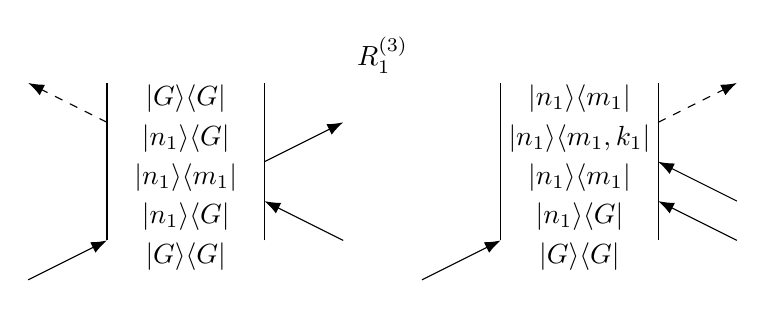
\begin{tikzpicture}[x=.5cm,y=.5cm]
\node[above] at (7, 4) {$R_{1}^{(3)}$};
%stimulated emission
\draw (0,0) -- (0,4);
\draw (4,0) -- (4,4);
\draw[\arw] (-2,-1) -- (0 ,0);
\draw[\arw] ( 6, 0) -- (4, 1);
\draw[\arw] ( 4, 2) -- (6 ,3);
\draw[dashed,\arw] ( 0, 3) -- (-2,4);
\node[above] at (2,-1) {\ket{G}\bra{G}};
\node[above] at (2, 0) {\ket{n_{1}}\bra{G}};
\node[above] at (2, 1) {\ket{n_{1}}\bra{m_{1}}};
\node[above] at (2, 2) {\ket{n_{1}}\bra{G}};
\node[above] at (2, 3) {\ket{G}\bra{G}};
%excited state absorption
\draw (10,0) -- (10,4);
\draw (14,0) -- (14,4);
\draw[\arw] ( 8,-1)  -- (10 ,0);
\draw[\arw] (16, 0)  -- (14, 1);
\draw[\arw] (16, 1)  -- (14, 2);
\draw[dashed,\arw] (14, 3)  -- (16, 4);
\node[above] at (12,-1) {\ket{G}\bra{G}};
\node[above] at (12, 0) {\ket{n_{1}}\bra{G}};
\node[above] at (12, 1) {\ket{n_{1}}\bra{m_{1}}};
\node[above] at (12, 2) {\ket{n_{1}}\bra{m_{1},k_{1}}};
\node[above] at (12, 3) {\ket{n_{1}}\bra{m_{1}}};
\end{tikzpicture}

\vspace{.5cm}

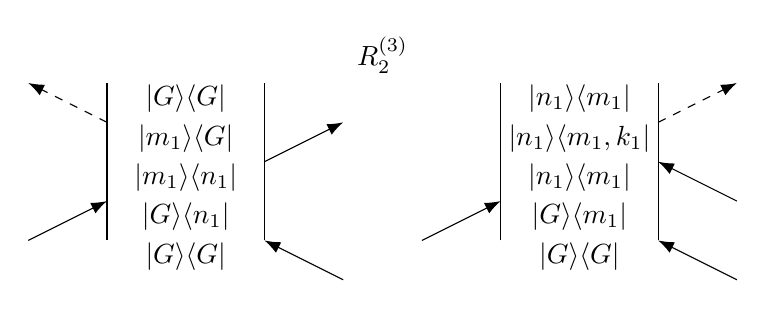
\begin{tikzpicture}[x=.5cm,y=.5cm]
\node[above] at (7, 4) {$R_{2}^{(3)}$};
%stimulated emission
\draw (0,0) -- (0,4);
\draw (4,0) -- (4,4);
\draw[\arw] ( 6,-1) -- (4 ,0);
\draw[\arw] (-2, 0) -- (0, 1);
\draw[\arw] ( 4, 2) -- (6 ,3);
\draw[dashed,\arw] ( 0, 3) -- (-2,4);
\node[above] at (2,-1) {\ket{G}\bra{G}};
\node[above] at (2, 0) {\ket{G}\bra{n_{1}}};
\node[above] at (2, 1) {\ket{m_{1}}\bra{n_{1}}};
\node[above] at (2, 2) {\ket{m_{1}}\bra{G}};
\node[above] at (2, 3) {\ket{G}\bra{G}};
%excited state absorption
\draw (10,0) -- (10,4);
\draw (14,0) -- (14,4);
\draw[\arw] (16,-1)  -- (14 ,0);
\draw[\arw] ( 8, 0)  -- (10, 1);
\draw[\arw] (16, 1)  -- (14, 2);
\draw[dashed,\arw] (14, 3)  -- (16, 4);
\node[above] at (12,-1) {\ket{G}\bra{G}};
\node[above] at (12, 0) {\ket{G}\bra{m_{1}}};
\node[above] at (12, 1) {\ket{n_{1}}\bra{m_{1}}};
\node[above] at (12, 2) {\ket{n_{1}}\bra{m_{1},k_{1}}};
\node[above] at (12, 3) {\ket{n_{1}}\bra{m_{1}}};
\end{tikzpicture}

\vspace{.5cm}

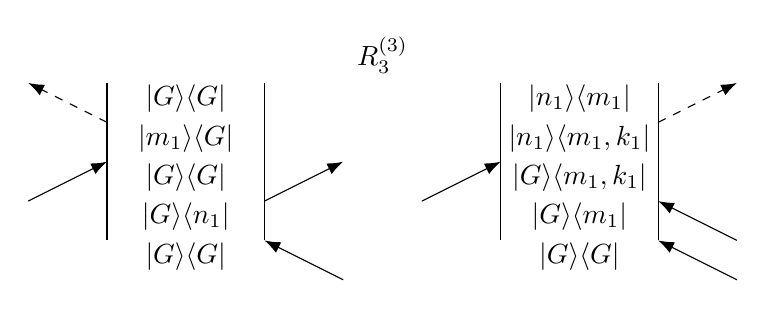
\begin{tikzpicture}[x=.5cm,y=.5cm]
\node[above] at (7, 4) {$R_{3}^{(3)}$};
%ground state bleach
\draw (0,0) -- (0,4);
\draw (4,0) -- (4,4);
\draw[\arw] ( 6,-1) -- (4 ,0);
\draw[\arw] ( 4, 1) -- (6, 2);
\draw[\arw] ( -2, 1) -- (0 ,2);
\draw[dashed,\arw] ( 0, 3) -- (-2,4);
\node[above] at (2,-1) {\ket{G}\bra{G}};
\node[above] at (2, 0) {\ket{G}\bra{n_{1}}};
\node[above] at (2, 1) {\ket{G}\bra{G}};
\node[above] at (2, 2) {\ket{m_{1}}\bra{G}};
\node[above] at (2, 3) {\ket{G}\bra{G}};
%excited state absorption
\draw (10,0) -- (10,4);
\draw (14,0) -- (14,4);
\draw[\arw] (16,-1)  -- (14 ,0);
\draw[\arw] (16, 0)  -- (14, 1);
\draw[\arw] (8, 1)  -- (10, 2);
\draw[dashed,\arw] (14, 3)  -- (16, 4);
\node[above] at (12,-1) {\ket{G}\bra{G}};
\node[above] at (12, 0) {\ket{G}\bra{m_{1}}};
\node[above] at (12, 1) {\ket{G}\bra{m_{1},k_{1}}};
\node[above] at (12, 2) {\ket{n_{1}}\bra{m_{1},k_{1}}};
\node[above] at (12, 3) {\ket{n_{1}}\bra{m_{1}}};
\end{tikzpicture}

\vspace{.5cm}

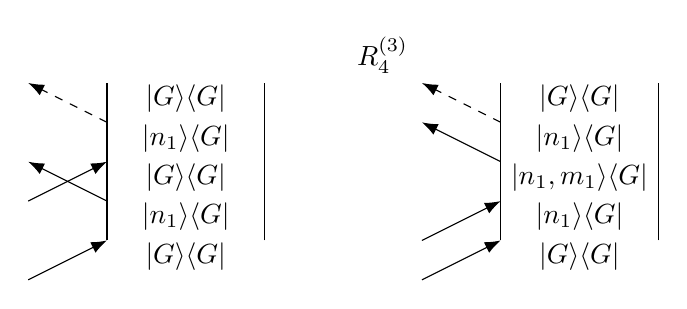
\begin{tikzpicture}[x=.5cm,y=.5cm]
\node[above] at (7, 4) {$R_{4}^{(3)}$};
%ground state bleach
\draw (0,0) -- (0,4);
\draw (4,0) -- (4,4);
\draw[\arw] ( -2,-1) -- (0 ,0);
\draw[\arw] (  0, 1) -- (-2, 2);
\draw[\arw] ( -2, 1) -- (0 ,2);
\draw[dashed,\arw] ( 0, 3) -- (-2,4);
\node[above] at (2,-1) {\ket{G}\bra{G}};
\node[above] at (2, 0) {\ket{n_{1}}\bra{G}};
\node[above] at (2, 1) {\ket{G}\bra{G}};
\node[above] at (2, 2) {\ket{n_{1}}\bra{G}};
\node[above] at (2, 3) {\ket{G}\bra{G}};
%excited state absorption
\draw (10,0) -- (10,4);
\draw (14,0) -- (14,4);
\draw[\arw] (8,-1)  -- (10 ,0);
\draw[\arw] (8, 0)  -- (10, 1);
\draw[\arw] (10, 2)  -- (8, 3);
\draw[dashed,\arw] (10, 3)  -- (8, 4);
\node[above] at (12,-1) {\ket{G}\bra{G}};
\node[above] at (12, 0) {\ket{n_{1}}\bra{G}};
\node[above] at (12, 1) {\ket{n_{1},m_{1}}\bra{G}};
\node[above] at (12, 2) {\ket{n_{1}}\bra{G}};
\node[above] at (12, 3) {\ket{G}\bra{G}};
\end{tikzpicture}
\caption{Two-sided Feynman diagrams for the third-order response function, as indicated.
For each $R^{(3)}$ the left diagram shows the one-exciton pathway and the right diagram shows the two-exciton pathway.
Note that we have labeled all doubly excited states as \bra{m_{1},k_{1}} indicating that two different chromophores are singly excited.
It is also possible that a single cromophore is doubly excited \bra{m_{2}}, but we have omitted this in the diagram for brevity.
Moreover, the doubly excited state is indicated to always return to the original singly excited state \bra{m_{1}}, but  it is also possible to return to a different singly excited state \bra{k_{1}}.
This is also omitted for brevity.}\label{fig:fd3}
\end{figure}

\clearpage
\section{Third-Order Response Functions -- Rephasing vs. Non-Rephasing}
The eight contributions to the third-order response functions are now classified as rephasing or non-rephasing and as either ground-state bleach, stimulated emission, excited state absorption, or two-quantum.\cite{Hamm2011}
Finally, we also rewrite the equations so that in the corresponding Feynman diagrams the last interaction gives emission from the ket (left), following the convention in Hamm and Zanni.\cite{Hamm2011}
This should make the numerical implementation of these equations more straightforward.

\subsection{Rephasing: Ground State Bleach}
\begin{figure}[h]
\centering
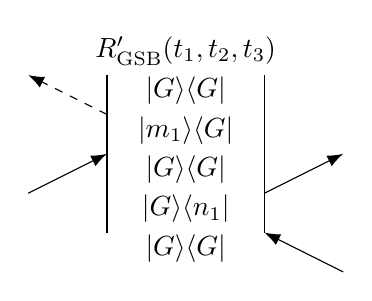
\begin{tikzpicture}[x=.5cm,y=.5cm]
\node[above] at (2, 4) {$R_\mathrm{GSB}'(t_{1},t_{2},t_{3})$};
%ground state bleach
\draw (0,0) -- (0,4);
\draw (4,0) -- (4,4);
\draw[\arw] ( 6,-1) -- (4 ,0);
\draw[\arw] ( 4, 1) -- (6, 2);
\draw[\arw] ( -2, 1) -- (0 ,2);
\draw[dashed,\arw] ( 0, 3) -- (-2,4);
\node[above] at (2,-1) {\ket{G}\bra{G}};
\node[above] at (2, 0) {\ket{G}\bra{n_{1}}};
\node[above] at (2, 1) {\ket{G}\bra{G}};
\node[above] at (2, 2) {\ket{m_{1}}\bra{G}};
\node[above] at (2, 3) {\ket{G}\bra{G}};
\end{tikzpicture}
\end{figure}
\begin{equation}
\begin{split}
 R_\mathrm{GSB}'(t_{1},t_{2},t_{3})=&\left\langle\underbar{\vect{M}}_{g1}^{T}[\vect q(\tau_{0})]\exp\left[i/\hbar\int_{\tau_{0}}^{\tau_{1}}\underbar{\vect{H}}^{1}[\vect q(\tau)]d\tau\right] \underbar{\vect{M}}_{g1} [\vect q(\tau_{1})]\right.\\
			  \times&\left.\underbar{\vect{M}}_{g1}^{T}[\vect q(\tau_{3})]\exp\left[-i/\hbar\int_{\tau_{2}}^{\tau_{3}}\underbar{\vect{H}}^{1}[\vect q(\tau)]d\tau\right] \underbar{\vect{M}}_{g1} [\vect q(\tau_{2})]\right\rangle_{b}
\end{split}
\end{equation}
The rephasing ground state bleach pathway is given by the one-exciton pathway of $R_{3}^{(3)}$.

\clearpage
\subsection{Rephasing: Stimulated Emission }
\begin{figure}[h]
\centering
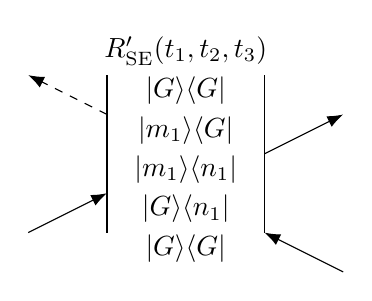
\begin{tikzpicture}[x=.5cm,y=.5cm]
\node[above] at (2, 4) {$R_\mathrm{SE}'(t_{1},t_{2},t_{3})$};
%stimulated emission
\draw (0,0) -- (0,4);
\draw (4,0) -- (4,4);
\draw[\arw] ( 6,-1) -- (4 ,0);
\draw[\arw] (-2, 0) -- (0, 1);
\draw[\arw] ( 4, 2) -- (6 ,3);
\draw[dashed,\arw] ( 0, 3) -- (-2,4);
\node[above] at (2,-1) {\ket{G}\bra{G}};
\node[above] at (2, 0) {\ket{G}\bra{n_{1}}};
\node[above] at (2, 1) {\ket{m_{1}}\bra{n_{1}}};
\node[above] at (2, 2) {\ket{m_{1}}\bra{G}};
\node[above] at (2, 3) {\ket{G}\bra{G}};
%excited state absorption
\end{tikzpicture}
\end{figure}
\begin{equation}
\begin{split}
 R_\mathrm{SE}'(t_{1},t_{2},t_{3})=&\left\langle\underbar{\vect{M}}_{g1}^{T}[\vect q(\tau_{0})]\exp\left[i/\hbar\int_{\tau_{0}}^{\tau_{2}}\underbar{\vect{H}}^{1}[\vect q(\tau)]d\tau\right] \underbar{\vect{M}}_{g1} [\vect q(\tau_{2})]\right.\\
			  \times&\left.\underbar{\vect{M}}_{g1}^{T}[\vect q(\tau_{3})]\exp\left[-i/\hbar\int_{\tau_{1}}^{\tau_{3}}\underbar{\vect{H}}^{1}[\vect q(\tau)]d\tau\right] \underbar{\vect{M}}_{g1} [\vect q(\tau_{1})]\right\rangle_{b}
\end{split}
\end{equation}
The rephasing stimulated emission pathway is given by the one-exciton pathway of $R_{2}^{(3)}$.

\subsection{Rephasing: Excited State Absorption}
\begin{figure}[h]
\centering
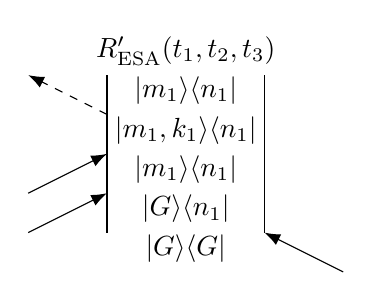
\begin{tikzpicture}[x=.5cm,y=.5cm]
\node[above] at (2, 4) {$R_\mathrm{ESA}'(t_{1},t_{2},t_{3})$};
%excited state absorption
\draw (0,0) -- (0,4);
\draw (4,0) -- (4,4);
\draw[\arw] ( 6,-1)  -- (4 ,0);
\draw[\arw] (-2, 0)  -- (0, 1);
\draw[\arw] (-2, 1)  -- (0, 2);
\draw[dashed,\arw] (0, 3)  -- (-2, 4);
\node[above] at (2,-1) {\ket{G}\bra{G}};
\node[above] at (2, 0) {\ket{G}\bra{n_{1}}};
\node[above] at (2, 1) {\ket{m_{1}}\bra{n_{1}}};
\node[above] at (2, 2) {\ket{m_{1},k_{1}}\bra{n_{1}}};
\node[above] at (2, 3) {\ket{m_{1}}\bra{n_{1}}};
\end{tikzpicture}
\end{figure}
\begin{equation}
\begin{split}
 R_\mathrm{ESA}'(t_{1},t_{2},t_{3})=-
			  &\left\langle\underbar{\vect{M}}_{g1}^{T}[\vect q(\tau_{1})]\exp\left[-i/\hbar\int_{\tau_{1}}^{\tau_{2}}\underbar{\vect{H}}^{1}[\vect q(\tau)]d\tau\right] \underbar{\vect{M}}_{12} [\vect q(\tau_{2})]\right.\\
			  &\times\exp\left[-i/\hbar\int_{\tau_{2}}^{\tau_{3}}\underbar{\vect{H}}^{2}[\vect q(\tau)]d\tau\right]\\
			  \times&\left.\underbar{\vect{M}}_{12}^{T}[\vect q(\tau_{3})]\exp\left[i/\hbar\int_{\tau_{0}}^{\tau_{3}}\underbar{\vect{H}}^{1}[\vect q(\tau)]d\tau\right] \underbar{\vect{M}}_{g1} [\vect q(\tau_{0})]\right\rangle_{b}.
\end{split}
\end{equation}
The rephasing excited state absorption pathway is given by the minus complex conjugate of the two-exciton pathway of $R_{1}^{(3)}$.\cite{Hamm2011}

\clearpage
\subsection{Non-Rephasing: Ground State Bleach}
\begin{figure}[h]
\centering
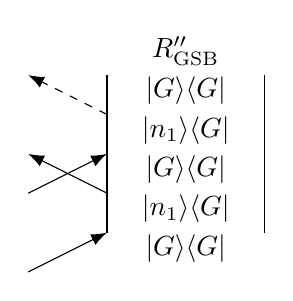
\begin{tikzpicture}[x=.5cm,y=.5cm]
\node[above] at (2, 4) {$R_\mathrm{GSB}''$};
%ground state bleach
\draw (0,0) -- (0,4);
\draw (4,0) -- (4,4);
\draw[\arw] ( -2,-1) -- (0 ,0);
\draw[\arw] (  0, 1) -- (-2, 2);
\draw[\arw] ( -2, 1) -- (0 ,2);
\draw[dashed,\arw] ( 0, 3) -- (-2,4);
\node[above] at (2,-1) {\ket{G}\bra{G}};
\node[above] at (2, 0) {\ket{n_{1}}\bra{G}};
\node[above] at (2, 1) {\ket{G}\bra{G}};
\node[above] at (2, 2) {\ket{n_{1}}\bra{G}};
\node[above] at (2, 3) {\ket{G}\bra{G}};
\end{tikzpicture}
\end{figure}
\begin{equation}
\begin{split}
 R_\mathrm{GSB}''(t_{1},t_{2},t_{3})=&\left\langle\underbar{\vect{M}}_{g1}^{T}[\vect q(\tau_{3})]\exp\left[-i/\hbar\int_{\tau_{2}}^{\tau_{3}}\underbar{\vect{H}}^{1}[\vect q(\tau)]d\tau\right] \underbar{\vect{M}}_{g1} [\vect q(\tau_{2})]\right.\\
			  \times&\left.\underbar{\vect{M}}_{g1}^{T}[\vect q(\tau_{1})]\exp\left[-i/\hbar\int_{\tau_{0}}^{\tau_{1}}\underbar{\vect{H}}^{1}[\vect q(\tau)]d\tau\right] \underbar{\vect{M}}_{g1} [\vect q(\tau_{0})]\right\rangle_{b}
\end{split}
\end{equation}
The non-rephasing ground state bleach pathway is given by the one-exciton pathway of $R_{4}^{(3)}$.

\subsection{Non-Rephasing: Stimulated Emission}
\begin{figure}[h]
\centering
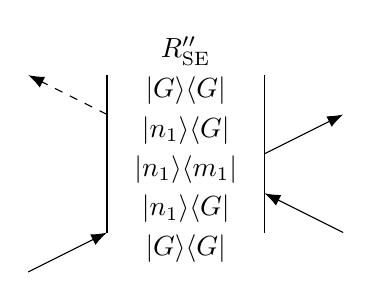
\begin{tikzpicture}[x=.5cm,y=.5cm]
\node[above] at (2, 4) {$R''_\mathrm{SE}$};
%stimulated emission
\draw (0,0) -- (0,4);
\draw (4,0) -- (4,4);
\draw[\arw] (-2,-1) -- (0 ,0);
\draw[\arw] ( 6, 0) -- (4, 1);
\draw[\arw] ( 4, 2) -- (6 ,3);
\draw[dashed,\arw] ( 0, 3) -- (-2,4);
\node[above] at (2,-1) {\ket{G}\bra{G}};
\node[above] at (2, 0) {\ket{n_{1}}\bra{G}};
\node[above] at (2, 1) {\ket{n_{1}}\bra{m_{1}}};
\node[above] at (2, 2) {\ket{n_{1}}\bra{G}};
\node[above] at (2, 3) {\ket{G}\bra{G}};
\end{tikzpicture}
\end{figure}
\begin{equation}
\begin{split}
 R_\mathrm{SE}''(t_{1},t_{2},t_{3})=&\left\langle\underbar{\vect{M}}_{g1}^{T}[\vect q(\tau_{1})]\exp\left[i/\hbar\int_{\tau_{1}}^{\tau_{2}}\underbar{\vect{H}}^{1}[\vect q(\tau)]d\tau\right] \underbar{\vect{M}}_{g1} [\vect q(\tau_{2})]\right.\\
			  \times&\left.\underbar{\vect{M}}_{g1}^{T}[\vect q(\tau_{3})]\exp\left[-i/\hbar\int_{\tau_{0}}^{\tau_{3}}\underbar{\vect{H}}^{1}[\vect q(\tau)]d\tau\right] \underbar{\vect{M}}_{g1} [\vect q(\tau_{0})]\right\rangle_{b}
\end{split}
\end{equation}
The non-rephasing stimulated emission pathway is given by the one-exciton pathway of $R_{1}^{(3)}$.

\clearpage
\subsection{Non-Rephasing: Excited State Absorption}
\begin{figure}[h]
\centering
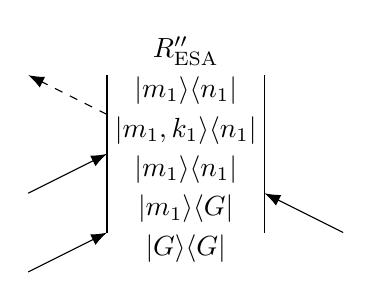
\begin{tikzpicture}[x=.5cm,y=.5cm]
\node[above] at (2, 4) {$R''_\mathrm{ESA}$};
%excited state absorption
\draw (0,0) -- (0,4);
\draw (4,0) -- (4,4);
\draw[\arw] (-2,-1)  -- (0 ,0);
\draw[\arw] ( 6, 0)  -- (4, 1);
\draw[\arw] (-2, 1)  -- (0, 2);
\draw[dashed,\arw] (0, 3)  -- (-2, 4);
\node[above] at (2,-1) {\ket{G}\bra{G}};
\node[above] at (2, 0) {\ket{m_{1}}\bra{G}};
\node[above] at (2, 1) {\ket{m_{1}}\bra{n_{1}}};
\node[above] at (2, 2) {\ket{m_{1},k_{1}}\bra{n_{1}}};
\node[above] at (2, 3) {\ket{m_{1}}\bra{n_{1}}};
\end{tikzpicture}
\end{figure}
\begin{equation}
\begin{split}
 R_\mathrm{ESA}''(t_{1},t_{2},t_{3})=-
			  &\left\langle\underbar{\vect{M}}_{g1}^{T}[\vect q(\tau_{0})]\exp\left[-i/\hbar\int_{\tau_{0}}^{\tau_{2}}\underbar{\vect{H}}^{1}[\vect q(\tau)]d\tau\right] \underbar{\vect{M}}_{12} [\vect q(\tau_{2})]\right.\\
			  &\times\exp\left[-i/\hbar\int_{\tau_{2}}^{\tau_{3}}\underbar{\vect{H}}^{2}[\vect q(\tau)]d\tau\right]\\
			  \times&\left.\underbar{\vect{M}}_{12}^{T}[\vect q(\tau_{3})]\exp\left[i/\hbar\int_{\tau_{1}}^{\tau_{3}}\underbar{\vect{H}}^{1}[\vect q(\tau)]d\tau\right] \underbar{\vect{M}}_{g1} [\vect q(\tau_{1})]\right\rangle_{b}
\end{split}
\end{equation}
The non-rephasing excited state absorption pathway is given by the minus complex conjugate of the two-exciton pathway of $R_{2}^{(3)}$.\cite{Hamm2011}

\subsection{Non-Rephasing: Two Quantum I}
\begin{figure}[h]
\centering
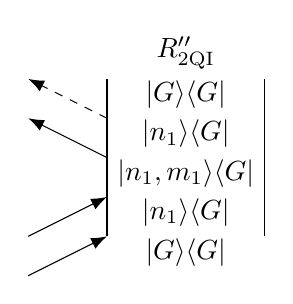
\begin{tikzpicture}[x=.5cm,y=.5cm]
\node[above] at (2, 4) {$R''_\mathrm{2QI}$};
%two-quantum
\draw (0,0) -- (0,4);
\draw (4,0) -- (4,4);
\draw[\arw] (-2,-1)  -- ( 0 ,0);
\draw[\arw] (-2, 0)  -- ( 0, 1);
\draw[\arw] ( 0, 2)  -- (-2, 3);
\draw[dashed,\arw] ( 0, 3)  -- (-2, 4);
\node[above] at (2,-1) {\ket{G}\bra{G}};
\node[above] at (2, 0) {\ket{n_{1}}\bra{G}};
\node[above] at (2, 1) {\ket{n_{1},m_{1}}\bra{G}};
\node[above] at (2, 2) {\ket{n_{1}}\bra{G}};
\node[above] at (2, 3) {\ket{G}\bra{G}};
\end{tikzpicture}
\end{figure}
\begin{equation}
\begin{split}
 R''_\mathrm{2QI}(t_{1},t_{2},t_{3})=
			  &\left\langle\underbar{\vect{M}}_{g1}^{T}[\vect q(\tau_{3})]\exp\left[-i/\hbar\int_{\tau_{2}}^{\tau_{3}}\underbar{\vect{H}}^{1}[\vect q(\tau)]d\tau\right] \underbar{\vect{M}}_{12} [\vect q(\tau_{2})]\right.\\
			  &\times\exp\left[-i/\hbar\int_{\tau_{1}}^{\tau_{2}}\underbar{\vect{H}}^{2}[\vect q(\tau)]d\tau\right]\\
			  \times&\left.\underbar{\vect{M}}_{12}^{T}[\vect q(\tau_{1})]\exp\left[-i/\hbar\int_{\tau_{0}}^{\tau_{1}}\underbar{\vect{H}}^{1}[\vect q(\tau)]d\tau\right] \underbar{\vect{M}}_{g1} [\vect q(\tau_{0})]\right\rangle_{b}
\end{split}
\end{equation}
The non-rephasing two quantum I pathway is given by the two-exciton pathway of $R_{4}^{(3)}$.

\clearpage
\subsection{Non-Rephasing: Two Quantum II}
\begin{figure}[h]
\centering
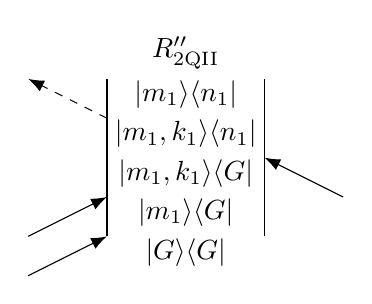
\begin{tikzpicture}[x=.5cm,y=.5cm]
\node[above] at (2, 4) {$R''_\mathrm{2QII}$};
%two-quantum
\draw (0,0) -- (0,4);
\draw (4,0) -- (4,4);
\draw[\arw] (-2,-1)  -- (0 ,0);
\draw[\arw] (-2, 0)  -- (0, 1);
\draw[\arw] (6, 1)  -- (4, 2);
\draw[dashed,\arw] (0, 3)  -- (-2, 4);
\node[above] at (2,-1) {\ket{G}\bra{G}};
\node[above] at (2, 0) {\ket{m_{1}}\bra{G}};
\node[above] at (2, 1) {\ket{m_{1},k_{1}}\bra{G}};
\node[above] at (2, 2) {\ket{m_{1},k_{1}}\bra{n_{1}}};
\node[above] at (2, 3) {\ket{m_{1}}\bra{n_{1}}};
\end{tikzpicture}
\end{figure}
\begin{equation}
\begin{split}
 R''_\mathrm{2QII}(t_{1},t_{2},t_{3})=-
			  &\left\langle\underbar{\vect{M}}_{g1}^{T}[\vect q(\tau_{0})]\exp\left[-i/\hbar\int_{\tau_{0}}^{\tau_{1}}\underbar{\vect{H}}^{1}[\vect q(\tau)]d\tau\right] \underbar{\vect{M}}_{12} [\vect q(\tau_{1})]\right.\\
			  &\times\exp\left[-i/\hbar\int_{\tau_{1}}^{\tau_{3}}\underbar{\vect{H}}^{2}[\vect q(\tau)]d\tau\right]\\
			  \times&\left.\underbar{\vect{M}}_{12}^{T}[\vect q(\tau_{3})]\exp\left[i/\hbar\int_{\tau_{2}}^{\tau_{3}}\underbar{\vect{H}}^{1}[\vect q(\tau)]d\tau\right] \underbar{\vect{M}}_{g1} [\vect q(\tau_{2})]\right\rangle_{b}.
\end{split}
\end{equation}
The non-rephasing two quantum II pathway is given by the minus complex conjugate of the two-exciton pathway of $R_{3}^{(3)}$.\cite{Hamm2011}

\clearpage
\section{Numerical Estimation of Exponential Integrals}
Following Jansen and Knoester,\cite{Jansen2006} the exponential integral operators, or propigators, can be estimated numerically by breaking them into a series of short intervals, during which the Hamiltonian is assumed constant
\begin{equation}
\begin{split}
\exp\left[-i/\hbar\int_{t_{0}}^{t_{1}}H(\tau)d\tau\right]\approx&
\exp\left[-\frac{i}{\hbar}H(t_{1}-\Delta t)\Delta t\right]
\exp\left[-\frac{i}{\hbar}H(t_{1}-2\Delta t)\Delta t\right]
\ldots\\
&\exp\left[-\frac{i}{\hbar}H(t_{0}+\Delta t)\Delta t\right]
\exp\left[-\frac{i}{\hbar}H(t_{0})\Delta t\right].
\end{split}
\end{equation}
The complex conjugate is given by the ususal rules of matrix multiplication
\begin{equation}
\begin{split}
\left(\exp\left[-i/\hbar\int_{t_{0}}^{t_{1}}H(\tau)d\tau\right]\right)^{*}\approx&
\left(\exp\left[-\frac{i}{\hbar}H(t_{1}-\Delta t)\Delta t\right]
\exp\left[-\frac{i}{\hbar}H(t_{1}-2\Delta t)\Delta t\right]
\ldots\right.\\
&\left.\exp\left[-\frac{i}{\hbar}H(t_{0}+\Delta t)\Delta t\right]
\exp\left[-\frac{i}{\hbar}H(t_{0})\Delta t\right]\right)^{*}\\
=&\exp\left[\frac{i}{\hbar}H(t_{0})\Delta t\right]
\exp\left[\frac{i}{\hbar}H(t_{0}+\Delta t)\Delta t\right]
\ldots\\
&
\exp\left[\frac{i}{\hbar}H(t_{1}-2\Delta t)\Delta t\right]
\exp\left[\frac{i}{\hbar}H(t_{1}-\Delta t)\Delta t\right]\\
\approx&
\exp\left[i/\hbar\int_{t_{0}}^{t_{1}}H(\tau)d\tau\right]
\end{split}
\end{equation}
where we have taken into account the fact that the Hamiltonian is symmetric.


\clearpage
\bibliography{/home/hestand/Documents/Research/Bibliography/HestandBib}
\bibliographystyle{unsrt}


\end{document}